\documentclass[oneside]{book}

\usepackage{ctex}
\usepackage{graphicx}
\usepackage{geometry}
\usepackage[hidelinks]{hyperref}
\usepackage{xcolor}
\usepackage{listings}
\hypersetup{
  colorlinks,
  citecolor=violet,
  linkcolor=gray,
  urlcolor=blue}
\geometry{a4paper,scale=0.8}

\title{华东师范大学算法分析助教简易手册}
\author{\href{mailto:zhzhwz@foxmail.com}{zhzhwz@foxmail.com}}

\begin{document}

\frontmatter

\maketitle

\chapter{前言}

\noindent \textbf{简介}

本手册为华东师范大学算法分析课程的助教编写,包含助教工作中可能涉及的各项流程和注意事项。

\bigbreak

\noindent \textbf{章节介绍}

第 \ref{chap:eoj} 章介绍了 EOJ 的使用方法,着重介绍了 EOJ Polygon 的使用。读者应先阅读前两节,按需阅读第 \ref{sec:polygon_operating_procedures} 节。

第 \ref{chap:elearning} 章介绍了大夏学堂的使用方法。该章暂时仅有少量工作建议,无具体操作流程。

第 \ref{chap:workflow} 章介绍了一些常见的工作流程,读者可在需要完成相应工作时参阅。

\bigbreak

\noindent \textbf{更多}

欢迎在本文的\href{https://github.com/zhzhwz/AlgorithmTAManual}{仓库}提交 issue 或 PR,促进本文的完善。

若遇到无法解决的问题,可在本文的\href{https://github.com/zhzhwz/AlgorithmTAManual}{仓库}提交 issue 或直接\href{mailto:zhzhwz@foxmail.com}{邮件联系作者}。 

若需要其他相关材料(包括各类文档的源文件,各类源代码等),请联系老师或作者。联系作者时请提供简要的身份证明,以避免材料外泄,对教学工作产生影响。

\tableofcontents

\mainmatter

\chapter{EOJ}

\label{chap:eoj}

\section{EOJ 基础}

ECNU Online Judge (EOJ) 是由华东师范大学已毕业的学长开发的在线评测系统。

\subsection{EOJ 的网址}

\href{https://acm.ecnu.edu.cn/}{https://acm.ecnu.edu.cn/}

\subsection{EOJ 的基础用法}

% TODO: add details

请自行摸索或联系作者获取更多信息(我不觉得作者能给你比自行摸索能得到的更多的信息)。

\section{EOJ Polygon 基础}

EOJ Polygon 是 EOJ 的『题目与比赛管理子系统』。

\subsection{如何获取 EOJ Polygon 权限}

\label{ssec:eoj_polygon_permission}

普通用户没有使用 EOJ Polygon 的权限。你需要联系 EOJ 的管理员以获取权限。以下是可能的寻找 EOJ 管理员的方式:

\begin{itemize}
    \item 在 EOJ 主页上寻找管理团队的联系方式(目前为 \href{mailto:acmsupport@admin.ecnu.edu.cn}{acmsupport@admin.ecnu.edu.cn}),联系时表明你的身份和需求(即,需要 EOJ Polygon 的权限),提供你的 EOJ 用户名。(推荐)
    \item 找你的课程老师,让他帮你联系算法竞赛团队的老师要权限
    \item 在 EOJ QQ 群(当前群号:691713742)中问谁是管理员(如果你是社牛可以考虑这个方案)
    \item 联系作者,作者帮你问(不推荐(如果实在不行就来问吧(叹气)))
\end{itemize}

\subsection{使用 EOJ Polygon}

在获取 Polygon 的权限后,你就可以在用户名的下拉菜单(如图 \ref{fig:polygon_entry_user})或者 EOJ 主页的最下方(如图 \ref{fig:polygon_entry_main_page})找到 Polygon 的入口了。EOJ 的主要创建人张羽戈在知乎写了一篇(并没有那么)详尽的文档,包含了几乎所有的 Polygon 的常见用法。详见:\href{https://zhuanlan.zhihu.com/p/59869879}{EOJ Polygon 使用指北 - 知乎}。

\begin{figure}[htbp]
  \centering
  \begin{minipage}{0.28\textwidth}
    \centering
    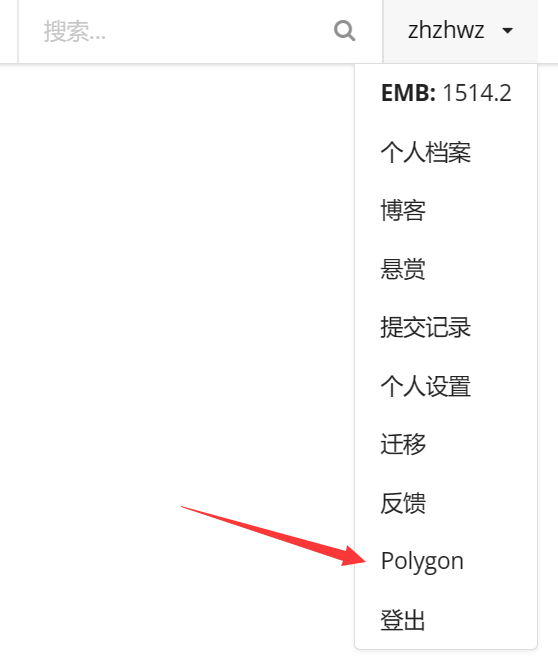
\includegraphics[width=\textwidth]{res/polygon_entry_user.png}
    \caption{用户名下拉菜单处 Polygon 入口}
    \label{fig:polygon_entry_user}
  \end{minipage}
  \begin{minipage}{0.7\textwidth}
    \centering
    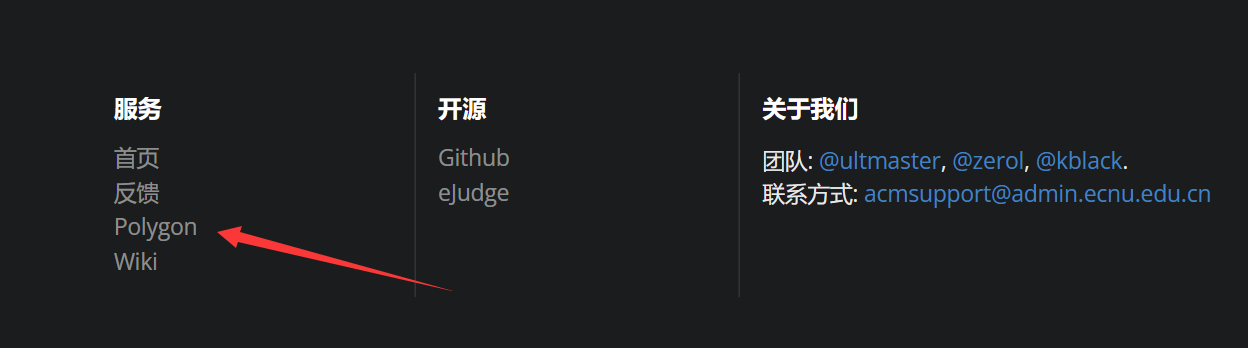
\includegraphics[width=\textwidth]{res/polygon_entry_main_page.png}
    \caption{EOJ 主页最下方处 Polygon 入口}
    \label{fig:polygon_entry_main_page}
  \end{minipage}
\end{figure}

\section{EOJ Polygon 相关常用操作流程}

\label{sec:polygon_operating_procedures}

\subsection{获取往届算法分析作业题和小测题的使用权限}

\label{ssec:permission_get}

以下是可能的方法:

\begin{itemize}
    \item 找你的课程老师,让他给你权限。前提是你的老师拥有对应作业集或比赛的权限。具体的操作步骤为:进入Polygon -- 比赛管理 -- 找到对应的作业集或比赛 -- 进入 -- 修改管理权限 -- 输入并选择要授予权限的用户 -- 点击``必须在这里保存''。
    \item 找作者要权限。前提是作者有权限。
    \item 如果想要其他作业集的权限,联系对应作业集或比赛的管理员,或直接联系 EOJ 的管理员(联系方法参见第 \ref{ssec:eoj_polygon_permission} 小节)。
\end{itemize}

\textbf{\textcolor{red}{注意:请务必在你创建的作业集或比赛中,在管理权限中加上你的老师。否则以后的助教就只能来找你要权限了。(你也可以在管理权限中加上作者(EOJ 用户名:zhzhwz))}}

\subsection{创建一个作业集或比赛}

\label{ssec:create_homework_set}

如图 \ref{fig:create_contest} 在 Polygon 中,进入比赛管理,选择 Add Contest,单击 Yes。系统会提示你创建比赛是无法撤销的,但由于比赛可以设置可见性,因此误创建也并不会产生过多影响。

\begin{figure}[htbp]
  \centering
  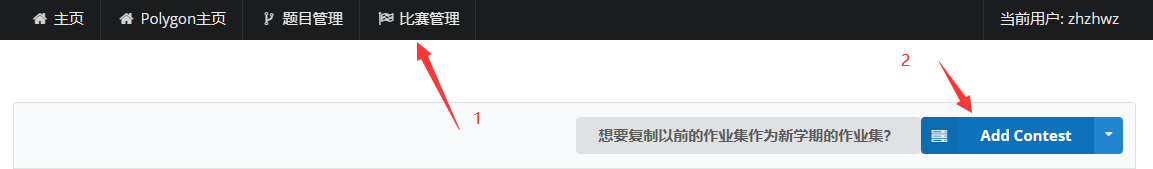
\includegraphics[width=\textwidth]{res/create_contest.png}
  \caption{创建比赛}
  \label{fig:create_contest}
\end{figure}

创建比赛后,需要对基本信息做一些修改。下面是一些比较重要的选项,更详细的信息请参见\href{https://zhuanlan.zhihu.com/p/59869879}{EOJ Polygon 使用指北 - 知乎}。

\begin{itemize}
  \item 修改管理权限:在这里,可以通过用户名搜索 EOJ 用户,授予他们对该场比赛的管理权限。添加完后,请立刻点击该栏下方的``必须在这里保存''。请注意,点击之后,该页面其他未保存的修改会被重置。因此,若该页有其他修改了未保存的项,请先点击页面最下方的确定保存修改,之后再添加管理员。一般来说,你应该将你的老师设为管理员。你也可以酌情将作者(zhzhwz)设为管理员。
  \item 标题:显示在作业集或者比赛栏中的标题。
  \item Allowed lang:允许学生提交的代码的语言类型。EOJ 目前(并在可预见的将来)不支持对比赛中某道题目设置允许的提交语言,也不允许对题目本身设置提交语言,而只能对一个作业集或比赛设置。
  \item Contest Type:设定该 Contest 为作业集或比赛。
  \item 时间设置、开始时间、结束时间:学生仅能在时间范围内提交代码。
  \item 访问控制:一般作业和小测都设置为``仅受邀用户可见,赛后题目不公开''。验题(详见第 \ref{sec:verify_problem} 节)用比赛一般设置为``仅比赛管理员可见'',并将所有验题人设置为管理员。
  \item 计分规则:一般用 OI 赛制,题目有部分分,无罚时。有需要可以使用 ACM 赛制,题目无部分分,有罚时。
  \item 允许代码共享:``代码在比赛过程中对 AC 用户公开''的意思是,若学生通过了一道题,那么他就能看到其他学生对该题的提交。不是很重要,如果有学生要求,可以开放。
  \item Case public:设为``评测报告总是开放''后,学生提交代码后,可以看到测试数据(若数据太大,则只能看到一部分)。若学生要求,可以在经老师同意后开放。(这可能能够帮助同学 debug,但也可能会导致成绩作弊。)
  \item 确定:点击后将会保存该页除``修改''栏的三项外的所有修改。请注意,该按钮与``修改''栏的三项下的``必须在这里保存''按钮分别是互斥的。即,点击任意一个按钮都会保存对应的信息,并将其他按钮对应的未保存的信息全部丢弃。
\end{itemize}

\subsection{导入学生名单}

\label{ssec:import_student_list}

在创建的比赛中,进入``邀请码''页面。点击``从名单导入''。你会看到提示:一行一个。这边每一行的信息会成为对某个学生的备注。一行的信息格式可以参照如下格式:

\begin{itemize}
  \item 学号\ 姓名\ 组号(若有)
\end{itemize}

例如:111 张三 1。

你可以在 Excel 中将这些信息填入不同的表格,之后直接复制即可。如图 \ref{fig:name_list_excel} 复制,粘贴后效果如图 \ref{fig:name_list_show}。

\begin{figure}[htbp]
  \centering
  \begin{minipage}{0.4\textwidth}
    \centering
    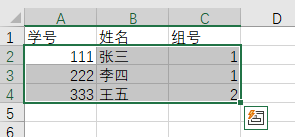
\includegraphics[width=\textwidth]{res/name_list_excel.png}
    \caption{Excel 中的信息}
    \label{fig:name_list_excel}
  \end{minipage}
  \hspace{0.1\textwidth}
  \begin{minipage}{0.4\textwidth}
    \centering
    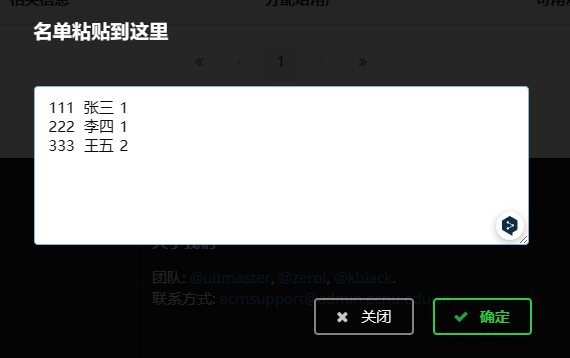
\includegraphics[width=\textwidth]{res/name_list_show.png}
    \caption{粘贴到 Polygon 后的信息}
    \label{fig:name_list_show}
  \end{minipage}
\end{figure}

你也可以根据实际情况设置信息的格式。

\subsection{导出邀请码}

\label{ssec:export_inviting_code}

在导入学生名单后,点击导出为 csv。为了使其能在微信等软件直接打开,你可能需要将其转为 xlsx 或 pdf 等其他文件格式。转为 pdf 时,记得检查有无出现字符重叠或部分字符未显示的情况。之后将文件发给同学即可。

\subsection{复制现有的题目}

\label{ssec:copy_exist_problem}

在 Polygon 题目管理中,选择 Request Clone。之后有三种情况:

\begin{itemize}
  \item 要复制的题目是你管理的比赛中的:这种情况下,按照提示输入 \lstinline{<ContestID>-<ProblemID>} 即可。
  \item 要复制的题目是公开题目集中的:首先任选一个你管理的比赛(或参考 \ref{ssec:create_homework_set} 创建一个),参考第 \ref{ssec:add_problem_to_homework_set} 小节将该题目添加到你管理的比赛。之后,按照上一条的方法处理即可。
  \item 都不是:联系题目或作业集的管理员,或者联系 EOJ 管理员(联系方式参见第 \ref{ssec:eoj_polygon_permission} 小节)请求获取权限。
\end{itemize}

\subsection{创建题目}

\label{ssec:create_new}

\subsection{将题目添加到作业集或比赛}

\label{ssec:add_problem_to_homework_set}

\subsection{更新题目}

\label{ssec:update_problem}

\subsection{重判题目}

\label{ssec:rejudge_problem}

\chapter{大夏学堂}

\label{chap:elearning}

% TODO: add details

大夏学堂有什么能讲的呢?自己摸索或者看大夏学堂的文档去吧。(主要是作者现在也登不进大夏学堂了)(欢迎补充该部分文档)

\section{工作建议}

\subsection{作业批改}

\begin{enumerate}
  \item 大夏学堂的作业批改功能存在许多问题,例如文件加载慢、批注框对中文支持很差(容易出现空格)等问题。建议的解决方案:将作业下载到本地分类,批改完后再将分数和批改意见依次填回。
  \item 批改时记录一下每次作业的易错点或常见问题,方便之后作业讲评时使用。
\end{enumerate}


\chapter{常见工作流程}

\label{chap:workflow}

\section{创建作业集}

% TODO: finish it
\begin{enumerate}
  \item 参考第 \ref{ssec:create_homework_set} 小节的方法创建作业集。
\end{enumerate}

\section{布置一次作业}

\label{sec:set_homework}

\begin{enumerate}
  \item 和老师沟通,确定本次作业的题数和每题的主题或涉及算法。
  \item 寻找相关题目。以下是可能的方法:
  \begin{itemize}
    \item 在之前的作业集中选择合适的题目。若无对应作业集权限,参考第 \ref{ssec:permission_get} 小小节的方法获得之前作业集的权限。
    \item 在 EOJ 公开题目中寻找相关题目。
    \item 在其他 OJ 获取题面和数据。作者已知目前唯一能够方便获取数据的 OJ 仅有 \href{https://loj.ac/}{LOJ} ,但其题目难度普遍偏高,请谨慎挑选。
    \item 在其他 OJ 获得题面,并自己造数据。包括但不限于\href{https://www.luogu.com.cn/}{洛谷}等 OJ 的题面可以直接在题目界面复制 markdown 源代码。造数据的方法可以参见第 \ref{sec:generating_data} 节。
    \item 从零开始自行创建题目。见第 \ref{chap:create_problem} 章。
  \end{itemize}
  \item 和老师沟通选定的题目是否合适。
  \item 复制现有的题目,见第 \ref{ssec:copy_exist_problem} 小节;或创建题目,见第 \ref{ssec:create_new} 小节。
  \item 将题目添加到作业集,见第 \ref{ssec:create_homework_set} 小节。
\end{enumerate}

\section{准备一次小测}

\begin{enumerate}
  \item 和老师沟通,确定小测的题量、算法、难度、是否需要原创题等信息。
  \item 参照第 \ref{ssec:create_homework_set} 节创建一个比赛。
  \item 寻找相关题目。具体方法参见第 \ref{sec:set_homework} 节。需要注意的是,小测题目对于原创性的要求会更高,请尽量保证每位参与的同学都没有做过原题。(考虑到小测的目的是检测同学们的学习成果,题目与作业中的题目有相似性是允许甚至鼓励的。)
  \item 和老师沟通选定的题目是否合适。
  \item 复制现有的题目,见第 \ref{ssec:copy_exist_problem} 小节;或创建题目,见第 \ref{ssec:create_new} 小节。
  \item 将题目添加到比赛,见第 \ref{ssec:create_homework_set} 小节。
  \item 若包含原创题,建议参考第 \ref{sec:verify_problem} 节邀请同学验题。
\end{enumerate}

\chapter{从零开始创建一道题}

\label{chap:create_problem}

本章的内容对于无算法竞赛基础的读者可能难度较大。考虑到实际工作中可能会用到,此处给出一些简单的指引。若读完仍感觉无从下手,请咨询身边的朋友(如,有算法竞赛经历或出题经历的同学等)。

除了本文外,你也可以参考一些网络上的资料,如\href{https://oi-wiki.org/contest/problemsetting/}{出题 - OI-Wiki}等。

% TODO: finish it

\section{编写题面}

\section{编写标程}

\section{造数据}

\label{sec:generating_data}

\section{测试部分分}

\section{验题}

\label{sec:verify_problem}

\end{document}
